\documentclass[12pt]{cornouaille}
\dscornouaille
\newcommand{\syst}[2]{\left\{\begin{array}{#1}#2\end{array}\right.}
\usepackage{draftwatermark}
%%%%%%%%%%%%%%%%%%%%%%%%%%%%%%%%%%%%%%%%%%%
%BAC BlANC
% Date - Obli ou Spé - Durée - Série - Coef - Nbre Exos
%%%%%%%%%%%%%%%%%%%%%%%%%%%%%%%%%%%%%%%%%%%

\newcommand{\BacBlanc}[6]{
\fexo{#4}{}{#1}
\SetWatermarkLightness{0.75}
\SetWatermarkAngle{30}
\SetWatermarkScale{2}
\SetWatermarkFontSize{2cm}
\SetWatermarkText{#2}
\bfseries
\begin{center}
	\LARGE{ BACCALAUR\'EAT BLANC - Lycée de Cornouaille}
	
	\vspace{1.5cm}
	
	\Large {#1}
	
	\vspace{1.5cm}
	
	\LARGE{MATH\'EMATIQUES}\\
	#2
	
	\vspace{1.5cm}
	
	\Large {Série #4}
	
	\vspace{1.5cm}
	
	Durée de l'épreuve: #3 \\
	Coefficient: #5
	
	\vspace{2cm}
	
	Les calculatrices sont autorisées,\\
	conformément à la réglementation en vigueur.
	
	\fbox{Le MODE EXAMEN est OBLIGATOIRE}
	
	\vspace{1.5cm}
	
	
	
\end{center}
\mdseries
Le sujet est composé de #6 exercices indépendants.Le candidat doit traiter tous les exercices.\\
Dans chaque exercice, le candidat peut admettre un résultat précédemment donné dans le texte pour aborder les questions suivantes, à condition de l'indiquer clairement sur la copie.\\
Le candidat est invité à faire figurer sur sa copie toute trace de recherche, même incomplète ou non fructueuse, qu'il aura développée.\\
Il est rappelé que la qualité de la rédaction, la clarté et la précision des raisonnements seront prises en compte dans l'appréciation des copies.

\begin{center}
	\textbf{Avant de composer, le candidat s'assurera que le sujet comporte bien 7 pages.}

\textbf{La page 7 est une annexe à rendre avec la copie.}
\end{center}



\newpage

\SetWatermarkText{}}

\begin{document}

\BacBlanc{Mars 2020 - 8h/12h}{Obligatoire}{4 heures}{S}{7}{4}



\begin{exercice}[Commun à  tous les candidats][5]
%Polynésie septembre 2019


\medskip

\emph{Pour chacune des cinq affirmations suivantes, indiquer si elle est vraie ou fausse, en justifiant la réponse.\\
Une réponse non justifiée n'est pas prise en compte.}

\medskip

\begin{enumerate}
\item On considère le nombre complexe $z = 1 + \text{i}\sqrt{3}$.\index{ecriture complexe@écriture complexe}

\smallskip

\textbf{Affirmation 1} : Le nombre complexe $z^2$ est un réel positif.

\setbar{1}
\begin{solution}
$z^2 = \left(1 + \text{i}\sqrt{3} \right)^2 = 1 - 3 + 2\text{i}\sqrt{3} = - 2 + 2\text{i}\sqrt{3} $ qui n'est pas un réel.
\end{solution}

\textbf{Affirmation 2} : L'argument du nombre complexe $z^{\np{2019}}$ vaut 0 modulo $2\pi$.

\setbar{1}
\begin{solution}
On a $|z|^2 = 1 + 3 = 4 = 2^2$, d'où $|z| = 2$. On peut en factorisant 2 écrire :

$z = 2\left( \dfrac{1}{2} + \text{i}\dfrac{\sqrt{3}}{2}\right) = 2\left( \cos \dfrac{\pi}{3} + \text{î}\sin \dfrac{\pi}{3}\right) = 2 \text{e}^{\text{i}\frac{\pi}{3}}$.

Il suit que  : $z^{\np{2019}} = \left[ 2 \text{e}^{\text{i}\frac{\pi}{3}} \right]^{\np{2019}} = 2^{\np{2019}} \text{e}^{\text{i}\frac{\np{2019}\pi}{3}} = \text{e}^{673\text{i}\pi}$.

Or $673\pi = 672\pi + \pi$ donc un argument de $z^{\np{2019}}$ est $\pi$ à $2\pi$ près.

L'affirmation est fausse.
\end{solution}
\end{enumerate}

Dans ce qui suit, le plan complexe est muni d'un repère orthonormé direct \Ouv.

\begin{enumerate}[resume]
\item On considère les points A, B et C d'affixes
respectives $z_{\text{A}} = \sqrt{2} + 3\text{i},\: z_{\text{B}} = 1 + \text{i}$ et $z_{\text{C}} = - 4\text{i}$.

\textbf{Affirmation 3} : Les points A, B et C ne sont pas alignés. %Polynésie 2016

\setbar{1}
\begin{solution}
Soit $Z=\dfrac{z_A-z_C}{z_B-z_C}=\dfrac{\sqrt{2}+7\text{i}}{1+5\text{i}}=\dfrac{1}{16}\left(\sqrt{2}+7\text{i} \right)\left(1-5\text{i} \right)=\dfrac{1}{16}\left(\vphantom{\dfrac{numérateur}{dénominateur}} (\sqrt{2}+35)+(7-5\sqrt{2})\text{i}\right) $

$Z \notin \R$ donc $arg(Z) \neq 0 (\pi)$ ~~~or~~~ $arg(Z)=arg\left(\dfrac{z_A-z_C}{z_B-z_C} \right)=\left(\vect{CB}~;~\vect{CA} \right) (2\pi)$

On en déduit que $\left(\vect{CB}~;~\vect{CA} \right) \neq 0 (\pi)$ donc $A~,~B~\text{et}~C$ ne sont pas alignés.

L'affirmation est VRAIE.
\end{solution}

\item On considère dans $\C$ l'équation $2z^2 - 3z + 5 = 0$.

\smallskip

\textbf{Affirmation 4} : Cette équation admet deux solutions dont les images sont symétriques par rapport à l'origine du repère.

\setbar{1}
\begin{solution}
On a $\Delta = 9 - 4 \times 2 \times 5 = 9 - 40 = - 31$ : cette équation a deux solutions complexes :

$z_1 - \dfrac{3 + \text{i}\sqrt{39}}{4}$\; \text{et }\; $z_1 - \dfrac{3 - \text{i}\sqrt{39}}{4}$ : les images de ces deux complexes sont symétriques autour de l'axe des abscisses. L'affirmation est fausse.
\end{solution}
\item  À tout point $M$ d'affixe $z$ du plan complexe, on associe le point $M'$ d'affixe $z'$  définie par :

\[z' = \overline{z}(1- z).\]

\textbf{Affirmation 5} : Il existe une infinité de points $M$ confondus avec leur point image $M'$.

\setbar{1}
\begin{solution}
$M = M' \iff z' = z = \overline{z}(1- z) $.

Avec $z = x + \text{i}y$, d'où $\overline{z} = x  - \text{i}y$, on obtient :

$z' = z \iff x + \text{i}y = ( x - \text{i}y)( 1 - x - \text{i}y) \iff x + \text{i}y = x(1 - x)  - y^2 + \text{i}[- xy + y(x - 1)]$.

En identifiant les parties réelles et imaginaires on obtient respectivement :

$\left\{\begin{array}{l c l}
x&=&x(1 - x) - y^2\\
y&=&- xy + y(x - 1)
\end{array}\right.$

La première équation donne $x^2 + y^2 = 0$, équation qui n'est vérifiée que par le couple (0~;~0).

La deuxième équation donne $y = -xy  + xy - y$ soit : $ 2y = 0$ d'où $y = 0$.

Les deux conditions devant être réalisées, le seul point confondu avec son image est l'origine O. L'affirmation est fausse.
\end{solution}
\end{enumerate}
\end{exercice}



\newpage


\begin{exercice}[Commun à tous les candidats][5]
%métropole juin 2016
	%\textbf{Pour les candidats n'ayant pas suivi l'enseignement de spécialité} 

\medskip

\textbf{Partie A}

\medskip

Soit $f$ la fonction définie sur $\R$ par 

\[f(x) = x - \ln \left(x^2 + 1\right).\]

\begin{enumerate}
\item Résoudre dans $R$ l'équation : $f(x) =x$.

\setbar{0.5}
\begin{solution}
Soit $x\in\R$ :

$\begin{array}[t]{llcl}
&f(x)&=&x\\
\iff&x-\ln(x^2+1)&=&x\\
\iff&\ln(x^2+1)&=&0\\
\iff&x^2+1&=&e^0\\
\iff&x^2&=&0\\
\iff&x&=&0\\
\end{array}$	
\[\text{L'équation }f(x)=x\text{ admet 0 pour unique solution}\]
\end{solution}
\item Justifier tous les éléments du tableau de variations ci-dessous à l'exception de la limite de la fonction $f$ en $+ \infty$ que l'on admet.

\begin{center}
\psset{unit=1cm}
\begin{pspicture}(9,3)
\psframe(9,3)\psline(0,2)(9,2)\psline(0,2.5)(9,2.5)\psline(1,0)(1,3)
\uput[u](0.5,2.4){$x$} \uput[u](1.4,2.4){$- \infty$} \uput[u](5,2.4){$1$} \uput[u](8.5,2.4){$+ \infty$} 
\rput(0.5,2.25){$f'(x)$}\rput(2.5,2.25){+} \rput(5,2.25){0}\rput(7,2.25){+}
\uput[u](1.5,0){$- \infty$}\uput[d](8.5,2){$+ \infty$}\rput(0.5,1){$f(x)$}
\psline{->}(2,0.3)(8,1.7)
\end{pspicture}
\end{center}

\setbar{1.5}
\begin{solution}
$\bullet\;$Montrons que $f$ est strictement croissante sur $\R$ :

La fonction $u : x\mapsto x^2+1$ est une fonction trinôme, donc dérivable là où elle est définie, i.e $\R$. 

Puisque $u>0$ sur $\R$, alors la fonction $\ln\circ u=\ln u$ est dérivable sur $\R$.

Finalement, la fonction $f$ est dérivable sur $\R$ comme différence des fonctions $x\mapsto x$ et $x\mapsto -\ln(x^2+1)$, toutes deux dérivables sur $\R$. Pour tout nombre réel $x$, on a :

\[f'(x)=1-\dfrac{2x}{x^2+1}=\dfrac{x^2+1-2x}{x^2+1}=\dfrac{(x-1)^2}{x^2+1}\]

La fonction $f$ est dérivable sur $\R$ et sa fonction dérivée est strictement positive sur $\R$, \emph{sauf pour $x=1$} : on en déduit que {\red $f$ est strictement croissante sur $\R$}. 
\par\medskip
$\bullet\;$Montrons $\lim_{x\to -\infty}f(x)=-\infty$ :

De $\syst{l}{\lim_{x\to -\infty}x^2+1=+\infty\\ \text{et}\\\lim_{X\to +\infty}\ln X=+\infty }$ on déduit, par composition : $\lim_{x\to -\infty}\ln(x^2+1)=+\infty$.

Il vient ensuite, par produit : \[\lim_{x\to -\infty}-\ln(x^2+1)=-\infty\]

De $\syst{l}{\lim_{x\to -\infty}x=-\infty\\ \text{et}\\\lim_{x\to -\infty}-\ln(x^2+1)=-\infty}$ on déduit, par somme : 

\[\lim_{x\to -\infty}f(x)=-\infty\]
\end{solution}
\item  Montrer que, pour tout réel $x$ appartenant à [0~;~1], $f(x)$ appartient à [0~;~1].

\setbar{0.5}
\begin{solution}
La  fonction $f$ est (strictement) croissante sur $[0,1]$. Par suite :
\[\forall x\in [0,1]\qquad f(0)\leqslant f(x)\leqslant f(1)\]
On a $\syst{l}{f(0)=0-\ln(0^2+1)=0\\ \text{et}\\ f(1)=1-\ln(1^2+1)=1-\ln 2}$. Puisque $1-\ln 2<1$, alors 
%$\ln 2>0$. On en déduit : $f(1)=1-\ln 2<1$.
%
%Puisque $\syst{l}{f(0)=0\\ \text{et}\\ f(1<1}$, on en déduit :
\[\forall x\in [0,1]\qquad 0\leqslant f(x)<1\]
On a prouvé :
\[ \forall x\in[0,1]\qquad f(x)\in[0,1]\]
\end{solution}
\item  On considère l'algorithme suivant :
\begin{center}
\begin{tabularx}{0.7\linewidth}{|l|X|}\hline
Variables 	&$N$ et $A$ des entiers naturels ;\\ \hline
Entrée 		&Saisir la valeur de $A$\\ \hline
Traitement 	&$N$ prend la valeur $0$\\
			&Tant que $N - \ln\left(N^2 + 1\right) < A$\\
			&\hspace{0,6cm}$N$ prend la valeur $N + 1$\\ 
			&Fin tant que\\ \hline
Sortie &Afficher $N$\\ \hline
\end{tabularx}
\end{center}
	\begin{enumerate}
		\item Que fait cet algorithme ?

\setbar{0.25}
\begin{solution}
L'algorithme affiche la plus petite valeur de $N$ pour laquelle $N-\ln(N^2+1)$ est supérieur ou égal à $N$.
\end{solution}
		\item Déterminer la valeur $N$ fournie par l'algorithme lorsque la valeur saisie pour $A$ est 100.

\setbar{0.25}
\begin{solution}
Pour $A=100$, l'algorithme affiche $110$
\end{solution}
 	\end{enumerate}
 \end{enumerate}
 
\bigskip

\textbf{Partie B}

\medskip

Soit $\left(u_n\right)$ la suite définie par $u_0 = 1$ et, pour tout entier naturel $n$, $u_{n+1} = u_n -\ln \left(u_n^2 + 1\right)$.

\medskip

\begin{enumerate}
\item Montrer par récurrence que, pour tout entier naturel $n$, $u_n$ appartient à [0~;~1].

\setbar{1}
\begin{solution}
Pour tout entier naturel $n$, notons $\mathcal{P}_n$ la propriété : $u_n\in[0,1]$.

$\bullet\;$ Puisque $u_0=1$, $\mathcal{P}_0$ est vraie.
\par\medskip
$\bullet\;$Supposons vraie la propriété $\mathcal{P}_n$ pour \emph{un} entier naturel $n$ quelconque. 

On a alors : $u_n \in [0~;~1]$.

D'après la troisième question de la partie A, on en déduit : 
\[f(u_n)\in[0~;~1]\]
soit :
\[u_{n+1}\in[0~;~1]\]	
On a prouvé :
\[\forall n\in\N\quad \mathcal{P}_n\text{ est vraie}\Longrightarrow\mathcal{P}_{n+1}\text{ est vraie}\]
\par\medskip
$\bullet\;$On a prouvé par récurrence :
\[ \forall n\in\N\qquad u_n\in[0~;~1]\]
\end{solution}
\item Étudier les variations de la suite $\left(u_n\right)$.

\setbar{0.5}
\begin{solution}
Soit $n\in\N$ :

$u_{n+1}-u_n=-\ln(u_n^2+1)$. 

Étudions le signe de $-\ln(u_n^2+1)$ :

Puisque $0\leqslant u_n\leqslant 1$, on en déduit, la fonction carré étant croissante sur $[0,1]$ : 
\[0^2\leqslant u_n ^2\leqslant 1^2\]
soit :
\[u_n^2\in[0~;~1]\]
Par suite :
\[u_n^2+1\in[1~;~2]\]
La fonction $\ln$ est croissante sur $[1~;~+\infty[$ : 

De $u_n^2+1\geqslant 1$, on déduit $\ln \left(u_n^2+1\right)\geqslant \ln 1$, soit $\ln \left(u_n^2+1\right)\geqslant 0$.

Puisque $u_{n+1} -  u_n = -\ln(u_n^2+1)\leqslant 0$, alors

\[\text{La suite $u$ est décroissante }\]
\end{solution}
\item Montrer que la suite $\left(u_n\right)$ est convergente.

\setbar{0.25}
\begin{solution}
La suite $u$ est décroissante et minorée par $0$ : elle converge donc, en vertu du théorème de la limite monotone, vers un nombre réel $\ell$.
\end{solution}
\item On note $\ell$ sa limite, et on admet que $\ell$ vérifie l'égalité $f(\ell) = \ell$.

En déduire la valeur de $\ell$.

\setbar{0.25}
\begin{solution}
Puisque l'équation $f(x) = x$ admet $0$ pour unique solution, on en déduit :
	\[ \ell = 0\]	
\end{solution}
\end{enumerate}
\end{exercice}

\newpage

\begin{exercice}[Commun à tous les candidats][5]
%Nouvelle Calédonie novembre 2016
%\textbf{Commun à tous les candidats}

\medskip

On considère le cube ABCDEFGH représenté ci-dessous.

On définit les points I et J respectivement par $\vect{\text{HI}} = \dfrac{3}{4} \vect{\text{HG}}$ et $\vect{\text{JG}} = \dfrac{1}{4} \vect{\text{CG}}$.

\begin{center}
\psset{unit=1cm}
\begin{pspicture}(8,8.25)
\psframe(0.5,0.5)(5,5)
\psline(5,0.5)(7,2.7)(7,7.2)(2.5,7.2)(0.5,5)
\psline(5,5)(7,7.2)
\psline[linestyle=dashed](0.5,0.5)(2.5,2.7)(7,2.7)
\psline[linestyle=dashed](2.5,2.7)(2.5,7.2)
\uput[ur](2.5,2.7){A} \uput[r](7,2.7){B} \uput[ul](5,0.5){C} 
\uput[ul](0.5,0.5){D} \uput[ul](2.5,7.2){E} \uput[ur](7,7.2){F} 
\uput[r](5,5){G} \uput[ul](0.5,5){H} \uput[u](3.875,5){I}
\psdots(5,0.5)(7,2.7)(7,7.2)(2.5,7.2)(0.5,5)(5,5)(3.875,5)(5,3.875)(2.5,2.7)(0.5,0.5) 
\uput[r](5,3.875){J} 
\end{pspicture}
\end{center}

\begin{enumerate}
\item \textbf{Sur le document réponse donné en annexe, à rendre avec la copie}, tracer, sans justifier, la section du cube par le plan (IJK) où K est un point du segment [BF].

\setbar{1}
\begin{solution}
On trace la section du cube par le plan (IJK):

\begin{center}
\psset{unit=1cm,PointSymbol=none,PointName=default,PtNameMath=false}
\begin{pspicture}(-1,-1)(7,6)
\pstGeonode[PosAngle=85](5.5,5){F}(1.5,5){E}(0,4){H}(4,4){G}
\pstGeonode[PosAngle=-70](0,0){D}(4,0){C}(5.5,1){B}(1.5,1){A}
\pstTranslation[DistCoef=.75,PosAngle=80,PointSymbol=*]{H}{G}{H}[I]
\pstTranslation[DistCoef=.75,PosAngle=10,PointSymbol=*]{C}{G}{C}[J]
\pstTranslation[DistCoef=.3,PosAngle=10,PointSymbol=*]{B}{F}{B}[K]
\psline(G)(H)(E)(F)(G)(C)(B)(F) \psline(C)(D)(H)
\psline[linestyle=dashed](D)(A)(B) \psline[linestyle=dashed](A)(E)
\psset{PointName=none}
\pstInterLL[PointSymbol=x]{J}{K}{F}{G}{M_1}
\pstLineAB[nodesep=-2,linestyle=dotted]{J}{K}
\pstLineAB[nodesep=-2,linestyle=dotted]{G}{F}
\pstInterLL[PointSymbol=x]{I}{M_1}{E}{F}{M_2}
\pstLineAB[nodesep=-2,linestyle=dotted]{I}{M_1}
\psset{linecolor=red,linewidth=1.5pt}
\pspolygon[style=TRed,linestyle=none](K)(J)(I)(M_2)
\psline(K)(J)(I)(M_2)
\psline[linestyle=dashed](M_2)(K)
\end{pspicture}
\end{center}
\end{solution}
\item \textbf{Sur le document réponse donné en annexe, à rendre avec la copie}, tracer, sans justifier, la section du cube par le plan (IJL) où L est un point de la droite (BF).

\setbar{1}
\begin{solution}
On trace la section du cube par le plan (IJL):

\begin{center}
\psset{unit=.9cm,PointSymbol=none,PointName=default,PtNameMath=false}
\begin{pspicture}(-.5,-1)(6,6)
\pstGeonode[PosAngle=85](1.5,5){E}(0,4){H}
\pstGeonode[PosAngle=-15](4,4){G}
\pstGeonode[PosAngle=40](5.5,5){F}(5.5,1){B}
\pstGeonode[PosAngle=-70](0,0){D}(4,0){C}(1.5,1){A}

\pstTranslation[DistCoef=.75,PosAngle=80,PointSymbol=*]{H}{G}{H}[I]
\pstTranslation[DistCoef=.75,PosAngle=10,PointSymbol=*]{C}{G}{C}[J]
\pstTranslation[DistCoef=.2,PosAngle=10,PointSymbol=*]{B}{F}{F}[L]
\psline(G)(H)(E)(F)(G)(C)(B)(F) \psline(C)(D)(H)
\psline[linestyle=dashed](D)(A)(B) \psline[linestyle=dashed](A)(E)
\pstLineAB[nodesep=-2]{F}{B}

\psset{PointName=none}
\pstInterLL[PointSymbol=x,PointName=M,PosAngle=-30]{J}{L}{G}{F}{M_1}
\pstLineAB[nodesep=-2,linestyle=dotted]{J}{L}
\psset{linecolor=red,linewidth=1.5pt}
\pspolygon[style=TRed,linestyle=none](I)(J)(M_1)
\psline(I)(J)(M_1)(I)
\end{pspicture}
\end{center}
\end{solution}
\item On se place dans le repère $\left(A;\vect{AB},\vect{AD},\vect{AE}\right)$.
\begin{enumerate}
	\item Donner, sans justifer, les coordonnées du point $J$.

\setbar{0.25}
\begin{solution}
$J \left(1,1,\frac{3}{4}\right)$
\end{solution}
	\item On admet que $I\left(\frac{3}{4};1;1\right)$ et $K\left(1;0;\frac{1}{3}\right)$.\newline
	Déterminer une représentation paramétrique de la droite $(IK)$.
	
\setbar{0.5}
\begin{solution}
$M(x,xy,z) \in (IK) \iff \exists t \in \R : \vect{KM}=t\vect{IK}$\\
$\iff \left\{\begin{array}{l c r}
x-1 &=& t(1-\frac{3}{4}) \\
y-0 &= & t(0-1) \\ 
z-\frac{1}{3} &=&t (\frac{1}{3}-1
 \end{array}\right.$ où $t \in \R$ $\iff \left\{\begin{array}{l c r}
x &=& \frac{1}{4}t + 1\\
y &= &-  t \\ 
z &=&-\frac{2}{3}t - \frac{1}{3}
 \end{array}\right.$ où $t \in \R$
\end{solution}
	\item On donne la droite $d$ de 
représentation paramétrique $\left\{\begin{array}{l c r}
x &=& 2t + 1\\
y &= &- 2 t + 9\\ 
z &=&t - 3
 \end{array}\right.$ où $t \in \R$.\newline
Le point $L(5~;~5~;~-1)$ appartient-il à $d$ ? Justifier.

\setbar{1}
\begin{solution}
On cherche s'il existe un réel t pour que les coordonnées du point $L$ vérifient le système: $\left\{\begin{array}{l c r}
5 &=& 2t + 1\\
5 &= &- 2 t + 9\\ 
-1 &=&t - 3
 \end{array}\right.$ soit $\left\{\begin{array}{l c r}
4 &=& 2t \\
-4 &= &- 2 t \\ 
2 &=&t 
 \end{array}\right.$ d'où $ t=2$ et oui le point appartient à la droite
\end{solution}
\item On donne la droite $\Delta$ de 
représentation paramétrique $\left\{\begin{array}{l c r}
x &=& -1-3t\\
y &= &7+t\\ 
z &=&-3-2t
 \end{array}\right.$ où $t \in \R$.\newline
Les droites $d$ et $\Delta$ sont-elles sécantes ? Si oui en quel point ?

\setbar{1}
\begin{solution}
On cherche s'il existent deux réels $t$ et $t'$ tels que :\\
$\left\{\begin{array}{l c r}
2t'+1 &=& -1-3t\\
-2t'+9 &= &7+t\\ 
t'-3 &=&-3-2t
 \end{array}\right. \iff \left\{\begin{array}{l c r}
2t'+3t &=& -2\\
-2t'+2 &= &t\\ 
t' &=&-2t
 \end{array}\right.\iff \left\{\begin{array}{l c r}
-4t+3t &=& -2\\
-2(2t)+2 &= &t\\ 
t' &=&-2t
 \end{array}\right.\iff \left\{\begin{array}{l c r}
t &=& 2\\
t &= &\frac{2}{5}\\ 
t' &=&-4
 \end{array}\right.$
le système n'admet pas de solution les deux droites ne sont pas sécantes.
%Sécantes en $L(5~;~5~;~-1)$ !!!! (mouhahahahahaha)
\end{solution}
	
\end{enumerate}
\end{enumerate}
	
\end{exercice}

\newpage

\begin{exercice}[Pour les candidats n'ayant pas suivi l'enseignement de spécialité][5]
%Métropole juin 2018
%\textbf{Commun à tous les candidats }

\bigskip

\emph{Les parties A et B de cet exercice sont indépendantes.}

\medskip

Le virus de la grippe atteint chaque année, en période hivernale, une partie de la population d'une ville.

La vaccination contre la grippe est possible; elle doit être renouvelée chaque année.

\bigskip

\textbf{Partie A}

\medskip

L'efficacité du vaccin contre la grippe peut être diminuée en fonction des caractéristiques
individuelles des personnes vaccinées, ou en raison du vaccin, qui n'est pas toujours
totalement adapté aux souches du virus qui circulent. Il est donc possible de contracter la
grippe tout en étant vacciné.

Une étude menée dans la population de la ville à l'issue de la période hivernale a permis de constater que :

\begin{itemize}
\item[$\bullet~~$]40\,\% de la population est vaccinée ;
\item[$\bullet~~$]8\,\% des personnes vaccinées ont contracté la grippe ;
\item[$\bullet~~$]20\,\% de la population a contracté la grippe.
\end{itemize}

\smallskip

On choisit une personne au hasard dans la population de la ville et on considère les
évènements :

\begin{description}
\item[ ] $V$ : << la personne est vaccinée contre la grippe >> ;
\item[ ] $G$ : << la personne a contracté la grippe >>.
\end{description}

\medskip

\begin{enumerate}
\item 
	\begin{enumerate}
		\item Donner la probabilité de l'évènement $G$.

\setbar{0.25}
\begin{solution}
$P(G)=0,2$ car 20\% de la population a contracté la grippe.
\end{solution}
		\item Reproduire l'arbre pondéré ci-dessous et compléter les pointillés indiqués sur quatre de ses branches.
		
		\begin{center}
\pstree[treemode=R,nodesepA=0pt,nodesepB=3pt]{\TR{}}
{\pstree{\TR{$V$~}\naput{\ldots}}
	{\TR{$G$}\naput{\ldots}
	\TR{$\overline{G}$}\nbput{\ldots}
	}
\pstree{\TR{$\overline{V}$~}\nbput{\ldots}}
	{\TR{$G$}
	\TR{$\overline{G}$}
	}
}	
		
		\end{center}

\setbar{0.5}
\begin{solution}
On obtient :
		\begin{center}
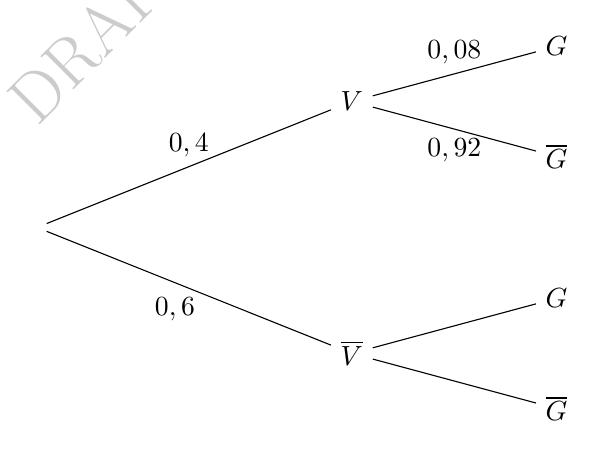
\begin{tikzpicture}[scale=2,grow'=right]  
\tikzstyle{level 1}=[sibling distance=16mm,level distance=20mm]  
\tikzstyle{level 2}=[sibling distance=7mm,level distance=13mm] 
\node{}  
	child{ node{$V$}
		child{ node{$G$} edge from parent node[above]{$0,08$} }
		child{ node{$\overline{G}$} edge from parent node[below]{$0,92$} }
		edge from parent node[above] {$0,4$}} 
	child{node{$\overline{V}$}
		child{ node{$G$} edge from parent node[above ] {$ $} }
		child{ node{$\overline{G}$} edge from parent node[below ] {$ $} }
		edge from parent node[below ] {$0,6 \quad$} };  
\end{tikzpicture}
\end{center}
\end{solution}
	\end{enumerate}
\item Déterminer la probabilité que la personne choisie ait contracté la grippe et soit vaccinée.

\setbar{0.25}
\begin{solution}
On calcule $P(G \cap V) = 0,4 \times 0,08 = 0,032$ soit $3,2\%$ de chances que la personne ait contractée la grippe et soit vaccinée.
\end{solution}
\item La personne choisie n'est pas vaccinée. Montrer que la probabilité qu'elle ait contracté la grippe est égale à $0,28$.

\setbar{0.75}
\begin{solution}
On calcule $P_{\overline{V}} (G) =\dfrac{P\left(\overline{V} \cap G\right) }{P\left(\overline{V}\right)}$\smallskip 
	
D'après la formule des probabilités totales, $P(V \cap G) + P\left(\overline{V} \cap G\right) = P\left(G\right)$.\smallskip 
	
Donc $P\left(\overline{V} \cap G\right) = P(G) - P(V \cap G) = 0,2 - 0,032 = 0,168$ puis $P_{\overline{V}} (G) = \dfrac{0,168}{0,6} =0,28$.

La probabilité qu'une personne non vaccinée ait contracté la grippe est égale à 0,28.
\end{solution}
\end{enumerate}

\bigskip

\textbf{Partie B}

\medskip

\emph{Dans cette partie, les probabilités demandées seront données à $10^{-3}$ près.}

\medskip

Un laboratoire pharmaceutique mène une étude sur la vaccination contre la grippe dans cette
ville.

\medskip

Après la période hivernale, on interroge au hasard $n$ habitants de la ville, en admettant que ce choix se ramène à $n$ tirages successifs indépendants et avec remise. On suppose que la probabilité qu'une personne choisie au hasard dans la ville soit vaccinée contre la grippe est égale à $0,4$.

On note $X$ la variable aléatoire égale au nombre de personnes vaccinées parmi les $n$
interrogées.

\medskip

\begin{enumerate}
\item Quelle est la loi de probabilité suivie par la variable aléatoire $X$ ?

\setbar{0.5}
\begin{solution}
Il s'agit de $n$ expériences aléatoires identiques et indépendantes à 2 issues (la personne est vaccinée ou non) avec une probabilité de succès de $0,4$.\smallskip 
	
La variable aléatoire $X$ compte le nombre de succès donc $X$ suit la loi binomiale $\mathcal{B}(n~;~0,4)$.
\end{solution}
\item Dans cette question, on suppose que $n = 40$.
	\begin{enumerate}
		\item Déterminer la probabilité qu'exactement $15$ des $40$ personnes interrogées soient vaccinées.

\setbar{0.25}
\begin{solution}
 $P(X=15) \approx 0,123$
\end{solution}
		\item Déterminer la probabilité qu'au moins la moitié des personnes interrogées soit vaccinée.

\setbar{0.5}	
\begin{solution}
$P(X \geqslant 20) = 1- P(X < 20) =  1- P(X \leqslant 19) \approx 0,130$
\end{solution}
 	\end{enumerate}
\item On s'intéresse à l'impact économique de la grippe sur la population active (personnes ayant un emploi).

D'après le réseau des GROG (Groupes Régionaux d'Observation de la Grippe),
le coût direct moyen d'un cas de grippe est de 70 euros (médecin + actes de soins + médicaments),
 auquel il faut ajouter les indemnités journalières d'absences (
	environ 4,8 jours d'absences en moyenne par personne
) soit 50 euros.

Par conséquent on peut estimer qu'un patient atteint de la grippe "coûte" 120 euros en frais de santé.

D'un autre coté, une vaccination contre la grippe coûte le prix du vaccin (7 euros),
 plus la consultation chez le médecin (23 euros),  soit 30 euros au total.

  \begin{enumerate}
  \item Quel est le coût en frais de santé d'une personne active qui s'est fait vacciner et qui contracte la grippe ?

\setbar{0.25}
\begin{solution}
$120+30=150$
\end{solution}
  \item On note $Z$ la variable aléatoire qui, à chaque personne active, associe le cout total de la grippe. 
  Donner sous forme de tableau la loi de probabilité de $Z$.

\setbar{0.5}
\begin{solution}
\begin{itemize}
	\item $P(Z=0) = P(\overline{V} \cap \overline{G})= 0,432$
	\item $P(Z=30)= P(V \cap \overline{G})=0,368$
	\item $P(Z=120)= P(\overline{V} \cap G)=0,168$
	\item $P(Z=150)= P(V \cap G)=0,032$
\end{itemize}

D'où la loi de probabilité de $Z$:


\begin{tabular}{|c|c|c|c|c|}
\hline
$z_i$ & 0     & 30    & 120   & 150   \\ \hline
$p_i$ & 0,432 & 0.368 & 0.168 & 0.032 \\ \hline
\end{tabular}

\end{solution}
  \item Quel est le coût moyen par personne active ?

\setbar{0.25}	
\begin{solution}
$E(Z) = 0.432 \times 0+0.368 \times 30+0.168 \times 120+0.032 \times 150=36$
\end{solution}


  \item En 2017, la France comptait environ 26,9 millions d'actifs\footnote{Source INSEE : https://www.insee.fr/fr/statistiques/3676623?sommaire=3696937} . Quel a été le coût total de la grippe en 2017 sur la population active ?

\setbar{0.25}
\begin{solution}
$26,9 \times 10^6 \times 36=968 \times 10^6$

Le coût a été de 968 millions d'euros, soit presque 1 milliards d'euros !
\end{solution}

  \end{enumerate}


\end{enumerate}

	
\end{exercice}

\newpage
\begin{center}

\textbf{À RENDRE AVEC LA COPIE}

\bigskip

\textbf{ANNEXE de l'exercice 3}

\bigskip

\textbf{Exercice 3, question 1}

\bigskip

\psset{unit=1cm}
\begin{pspicture}(8,8.25)
\psframe(0.5,0.5)(5,5)
\psline(5,0.5)(7,2.7)(7,7.2)(2.5,7.2)(0.5,5)
\psline(5,5)(7,7.2)
\psline[linestyle=dashed](0.5,0.5)(2.5,2.7)(7,2.7)
\psline[linestyle=dashed](2.5,2.7)(2.5,7.2)
\uput[ur](2.5,2.7){A} \uput[r](7,2.7){B} \uput[ul](5,0.5){C} 
\uput[ul](0.5,0.5){D} \uput[ul](2.5,7.2){E} \uput[ur](7,7.2){F} 
\uput[r](5,5){G} \uput[ul](0.5,5){H} \uput[u](3.875,5){I}\uput[r](7,3.7){K}
\psdots(5,0.5)(7,2.7)(7,7.2)(2.5,7.2)(0.5,5)(5,5)(3.875,5)(5,3.875)(2.5,2.7)(0.5,0.5)(7,3.7) 
\uput[r](5,3.875){J} 
\end{pspicture}

\bigskip

\textbf{Exercice 3, question 2}

\bigskip

\psset{unit=1cm}
\begin{pspicture}(0,-0.5)(8,9.25)
\psframe(0.5,0.5)(5,5)
\psline(5,0.5)(7,2.7)(7,7.2)(2.5,7.2)(0.5,5)
\psline(5,5)(7,7.2)\psline(7,-0.5)(7,9.25)
\psline[linestyle=dashed](0.5,0.5)(2.5,2.7)(7,2.7)
\psline[linestyle=dashed](2.5,2.7)(2.5,7.2)
\uput[ur](2.5,2.7){A} \uput[r](7,2.7){B} \uput[ul](5,0.5){C} 
\uput[ul](0.5,0.5){D} \uput[ul](2.5,7.2){E} \uput[ur](7,7.2){F} 
\uput[r](5,5){G} \uput[ul](0.5,5){H} \uput[u](3.875,5){I}\uput[r](7,8.4){L}
\psdots(5,0.5)(7,2.7)(7,7.2)(2.5,7.2)(0.5,5)(5,5)(3.875,5)(5,3.875)(2.5,2.7)(0.5,0.5)(7,8.4) 
\uput[r](5,3.875){J} 
\end{pspicture}
\end{center}
\end{document}